\chapter{Unassigned fieldstones}

\section{Bugs and flaws aren't limited to the app}
They're also in the environment, the tools used to measure, etc.


\section{On Devops and applying the mindset to Android apps using analytics tools}

Devops has become increasingly popular in industry. The mindset helps transform software development from Waterfall methodology (do each activity once, in sequence), through Agile (collaborate on smaller time-boxed sprints and aim to finish the work within that time-box) to developers being responsible for their software before and during production (\emph{i.e.} while it is being used in production. Devops seems to have been focused on online service providers and may also be highly relevant for in-house development team who provide internal online services.

DORA reports, Google Cloud \emph{"With over 70K downloads and input from 31K professionals worldwide, the Accelerate State of DevOps Report from DevOps Research and Assessment (DORA) is the longest running, academically rigorous research investigation into the capabilities and practices that make DevOps and transformation effective."}\url{https://cloud.google.com/devops/}

Applying devops to mobile (Android) apps. 

\section{Live Performances}
Some thoughts on how live performances are assessed to compare and contrast these with assessing the quality of Android apps.

Popularity measures: number of shows, length of runs of a play, etc. audience size, reviews (by critics and by the end users - the main audience) 

Behind the curtain measurements (that the crowd does not see and probably isn't aware of). timings, scenery changes, who actually performed and how well they fulfilled their obligations as musicians, actors, etc.

\section{What are we trying to measure?}
\emph{c.f. Google's earlier role of Software Quality Assurance Engineers and their associated roles}. How might we assess the quality of mobile apps using analytics?

\section{Fidelity}
\emph{"Success is built on trust."}

\emph{"Trust starts with transparency"}
\footnote{\url{https://trust.salesforce.com/en/}}

\begin{itemize}
    \item Model Fidelity and usefulness of the model(s). Models are not reality, nonetheless they may still be useful. Establishing a quality model using crashes and unresponsiveness data. Data collection, presentation, reporting.
    \item Stakeholders for the model and effects of the model for these stakeholders (including the app store, the developers and testing)
    \item Incomplete models, how well does the data represent the population and the quality characteristics of the software?
    \item (in)sufficiency of the data collected: how can the data be used, what are the limits? boundaries? transitional areas? Augmenting/enhancing the data collected using the current mechanism(s). Choosing additional/alternative mechanisms. (in)consistencies in the mechanisms. Privacy, performance, scope, etc. of various mechanisms.
    \item Gaming the model for fun and profit. Possible goals, mechanisms, etc. Discuss and provide examples of ways to game using various approaches (stop users from using the software, catch and discard errors (c.f. Blind SQL Injection story), change user's behaviour and/or expectations, implement alternatives, flood the database with positive data, fix the issue.
    \item Fool's Gold: of using crash rates, etc. as a measure of 'quality'. 
\end{itemize}

\section{Metrics}
\subsection{Vanity metrics?}
Public app store install count vs active install counts. Google Play Console describes 'Active installs' as  \textit{Installs on Active Devices (devices online in the past 30 days with this app installed).} As table \ref{tab:app_store_install_counts} shows the differences are significant, and the App Store Install count might seem to a vanity metric than anything else; nonetheless when combined with the install and uninstall reports high ratios (between the public and developer-centric counts) might indicate many users are rejecting the app. (There are probably other causes for users installing and uninstalling an app, for instance if they want to keep their devices clean, tidy, and performant; or if they only needed the app briefly for instance a local travel app such as `BVG FahrInfo Plus'\footnote{\url{ https://play.google.com/store/apps/details?id=de.eos.uptrade.android.fahrinfo.berlin}} used when visiting Berlin as a tourist. 
% TODO find an elegant way to shrink the line length of the long URL.

\begin{table}[]
\begin{tabular}{r|r|l}
\small
App Store Installs &Active Installs &App \\
\hline
500,000+     &149,192  &Kiwix \\
100,000+     &35,907  &Chemistry \& Physics simulations \\
500,000+     &138,350  &Moonpig \\
100,000+     &19,263  &Moodspace
\end{tabular}
\caption{App Store and Google Play Console counts}
\label{tab:app_store_install_counts}

\end{table}

\subsection{Estimating populations}


Percentages use a known denominator of 100 e.g. \( \frac{37}{100} \) and calculations of percentages are revised so that they use this denominator. For many of the reports, Google does not provide the denominator, for instance for crash clusters it provides the count of crashes on various devices, but not the total number of sessions, of users on that device. They do provide an overall percentage e.g. \texttt{95.4\%} crash-free sessions\footnote{Google Play Console describes these as: \textit{'Percentage of daily sessions between 2/4/19 and 5/5/19 during which your users did not experience any crashes. A daily session refers to a day during which your app was used.'}} and this may help us to estimate which devices are more likely to reproduce a crash once we can obtain and use data from other sources.

Here is the top crash cluster as an example:

\small{
\textbf{\texttt{java.lang.NullPointerException}}
\texttt{org.kiwix.kiwixmobile.downloader. \\ DownloadService.lambda\$updateDownloadFragmentProgress\$7}}
\normalsize

For this crash cluster, Google Play Console reports 209 crashes in the last 7 days; yet the totals of the 'By' charts are higher at 216 (By app version = 216, By Android version = 216, By device = 216). 

\begin{figure}
    \centering
    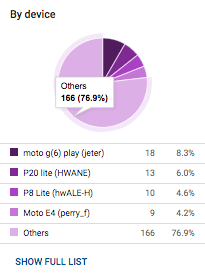
\includegraphics{images/ByDeviceNPE.png}
    \caption{By Device summary for the NullPointerException}
    \label{fig:device_summary_for_NPE}
\end{figure}
By device, in descending order, the crashes were:
\begin{center}
\begin{tabular}{l|r|r}
Device Model                    & Crashes & \\
\hline
moto g(6) play (jeter)	        & 18	& 8.3\% \\
P20 lite (HWANE)	            & 13	& 6.0\% \\
P8 Lite (hwALE-H)	            & 10	& 4.6\% \\
Moto E4 (perry\_f)	            & 9	    & 4.2\% \\
\textit{Others}\footnotemark    & 166 & 79.9\%  \\
\end{tabular}
\end{center}
\footnotetext{Can be expanded in the Google Dev Console's UI}
% For notes on how to create and format tables I started with https://www.overleaf.com/learn/latex/Tables and got the footnote in the table to appear once I separated the footnotemark from the footnotetext, see https://www.overleaf.com/learn/latex/Footnotes

% Thank you to https://www.overleaf.com/learn/latex/Fractions_and_Binomials for helping me learn how to write the following. Note: I'm sure the formatting and presentation can be improved significantly.
\(\frac{18}{?} \) \texttt{+} \(\frac{13}{?} \) \texttt{+} \(\frac{10}{?} \) \texttt{+} \(\frac{9}{?} \) \texttt{+} \(\frac{166}{?} \)  \texttt{=}  \(\frac{216}{?}\)

These are for the last 7 days; to get an accurate estimate of the crashes per device we need to pick the same period as Google uses for their calculation of 'daily sessions' i.e. \textbf{TODO once I've more examples: it seems to be around 3 calendar months though...}

Sum the crash counts by device model across the set of crash clusters. Add up the various crash counts (including those sum of those classified as `Other`). Then multiply the total: 

\textit{Total Sessions = sum of all crashes * } \(\frac{\textit{100}}{1 - crash-free\ daily\ sessions} \) 

to obtain the total (approximate) count of sessions. The accuracy will depend on how consistent and accurate Google are in their definitions/terms and their calculations. For now we'll assume a low-to-middling confidence interval in the results of our calculations and hope we'll obtain greater accuracy as we collect more data from various sources.

Now we can estimate the number of crass free sessions per crash cluster; note the estimates are likely to have high error-bars as the crash rates per crash cluster is unlikely to be uniform.

Google Play Console does not provide data on the popularity of our app(s) on particular device models. It may be possible to infer approximate popularities using data from various other sources, for instance from market-wide statistics and reports. The app could also be modified to collect the data (indeed it may already collect the data either directly or by using a third-party library such as those for Mobile Analytics).

\subsubsection{Sanity checks}
In figure \ref{fig:android_vitals_excessive_network_usage} there are an estimated 475K sessions between 15th May and 12th June 2019, approximately 17K sessions a day. Some additional details are available in various reports on the same webpage e.g. by Android version, reproduced in table \ref{tab:android_vitals_session_counts_by_android_version} (note the total, 474K, does not quite add up to 475K)

\begin{table}[]
    \centering
    \begin{tabular}{l|r}
    Android Version &Number of sessions \\
    \hline
    9     &\textasciitilde{}125K \\
    8.1   &\textasciitilde{}247K \\
    8     &\textasciitilde{}102K
    \end{tabular}
    \caption{Android Vitals sessions: by Android version}
    \label{tab:android_vitals_session_counts_by_android_version}
\end{table}
% Thank you to https://en.wikibooks.org/wiki/LaTeX/Special_Characters for helping me get the tilde to display.

\section{Software Tools}
\emph{Kindof a related work section? as we've developed several tools including some that overlap with these.}
Discuss the relevance of being able to capture, query, and monitor the device logs for testing Android apps generally. 

Some of the challenges of doing so for many people (testers more than developers as developers are working with logs anyway/already).

Data volumes, logs are short-lived, and they are on the device. 

\url{https://github.com/JakeWharton/pidcat} enables logs to be displayed consistently for named software packages (explain briefly why names are relevant and how the package names emerge for apps, etc.) even as the PID changes (again mention what PIDs are).


\section{Encyclopedia for Tunisia}
3 accounts each installed the app on a separate device (OnePlus 6, Android 9.0, Samsung S7 Android 8.0, LG K4 Android ???).

Checked Android Vitals, only 2 installs showed.

Checked phones on Saturday evening, the OnePlus6 had send diagnostics and usage option disabled, so we enabled it. Subsequently checked Android Vitals on Sunday and Monday \nth{18} November 2019 still only shows 2 installs on the Friday \nth{15}: one with Android 9.0 and the other with Android 8.0. What happened to the install on the LG device?

\section{Prior work to consider}
Back in 2013 I wrote a set of notes titled: Mobile Analytics possible sources \url{https://docs.google.com/document/d/17a0WexTybVcaDjto9gqpSRD_O4zminZ_PwCGjiPHUk8/edit}. I think it'll be worth me reviewing these notes as some of the material is probably still relevant for my thesis even though much has changed since then e.g. GDPR, new Mobile Analytics tools, changes of ownership and popularity, the launch of Android Vitals, etc.

The development of code to test count.ly and potentially other mobile analytics \url{https://code.google.com/archive/p/mobile-analytics-research/}

My Probation Report (Summer 2015). At least check the references and who's built on their work since then. C.f. Stefan Foell's work (he was one of my examiners). He last published in 2016 according to Google Scholar \url{https://scholar.google.com/scholar?as_ylo=2015&q=stefan+foell&hl=en&as_sdt=0,5}

Look at quoting from the one and only MobiData workshop \emph{MobiData '16: Proceedings of the First Workshop on Mobile Data}. The most relevant seems to be \emph{The Need to Account for Geographical Diversities in Mobile Data Research} \url{https://dl.acm.org/doi/abs/10.1145/2935755.2935761}

\section{Prior work on usage analysis}
\emph{Smartphone usage in the wild: a large-scale analysis of applications and context}\footnote{\url{https://scholar.google.com/scholar?cites=2770414575190984561\&as_sdt=2005\&sciodt=0,5\&hl=en}} is a well referenced paper with over 200 citations. Of these, there are several themes to research usage. Examples include where users are based \href{Investigating Country Differences in Mobile App User Behavior and Challenges for Software Engineering}{https://ieeexplore.ieee.org/abstract/document/6913003}. They discuss app store mining, mining activity logs, etc. amongst other related work. The authors identify several challenges for app developers (software engineers) including: app packaging requirements (which is effectively their advert to users in the app store), managing vast feature spaces (e.g. should developers tailor their apps to specific countries/locales?), meeting high quality expectations (here this intersects with my research), managing [the] app store dependency (including product line engineering c.f. kiwix custom apps), addressing price sensitivity (as this may affect the ratings and reviews and abandonment), and balancing ecosystem effects (what do users consider important in the app store ecosystem? e.g. ratings).

The places of our lives: Visiting patterns and automatic labeling from longitudinal smartphone data
TMT Do, D Gatica-Perez - IEEE Transactions on Mobile …, 2013 - ieeexplore.ieee.org
The location tracking functionality of modern mobile devices provides unprecedented
opportunity to the understanding of individual mobility in daily life. Instead of studying raw
geographic coordinates, we are interested in understanding human mobility patterns based …
  Cited by 97 Related articles All 7 versions
[PDF] rahmati.com

Studying smartphone usage: Lessons from a four-month field study
A Rahmati, L Zhong - IEEE Transactions on Mobile Computing, 2012 - ieeexplore.ieee.org
Many emerging mobile applications and services are based on smartphones. We have
performed a four-month field study of the adoption and usage of smartphone-based services
by 14 novice teenage users. From the field study, we present the application usage and …

\section{Some Concepts}
Testing and automated testing provide results in various forms e.g. the old junit approach of using a character to indicate the result of each individual test \texttt{.} for a test that passed, \texttt{F} for a test that failed. These may be aggregated for a set of tests, again junit provides a summary with counts of the tests that were run together with any failures, errors, etc. 

We rely on these test results to varying degrees to assess the quality of the combination of what was being tested and the testing itself (after all sometimes the faults are in the tests or the test execution environment rather than in the software or system being tested (a system includes software and other elements e.g. the configuration, the platform (e.g. the OS), external dependencies, etc.).

\section{The relevance of latency on actions}
User updates are bursty, with the median being 0 update events per day the \nth{90} percentile 180 update events, and the maximum 9445. The majority of updates within 7 days of an updated version of an app being released \textbf{TODO add evidence}

\texttt{quantile(installs.data\$Update.events, seq(0, 1, 0.01))}

If we can get feedback about quality issues sooner we may be able to address the issues sooner in terms of limiting the number of users affected \emph{e.g.} by pausing, suspending, or stopping a rollout of the newer release; by providing timely information, support and advice to users; and initiate the bug investigation and resolution sooner with the aim of fixing the underlying issue as quickly as practical and making the fix available to affected users in particular and the rest of the user-base generally.

The latency of information for various data sources varies by analytics tool and type of data. Some data and reports are updated in retard, and based on the timezone used by the analytics provider \emph{e.g.} Google uses Pacific Time zone for their data collection and reporting. 

\begin{itemize}
    \item Google Play Console Reports: TBC
    \item Fabric Crashlytics Daily Summary email: TBC
    \item Android Vitals - Crash and ANR data: TBC
    \item Crashlytics Graphs and Reports: TBC
\end{itemize}

Detecting problems is key to being able to identify and address them. Quality issues can be assumed in software, no one writes perfect software (c.f. Knuth's payment per bug) especially no-one that writes mobile apps. Developers are often aware and consciously write code that is run when some expected exceptions and other issues occur. Crashes are seldom triggered deliberately in apps, they occur when something happens at run-time that developers did not write code to cope with. Reported crashes are one way that quality flaws can be analysed. The frequency of crashes may also be relevant in various ways, such as:

\begin{itemize}
    \item MTBF
    \item 'success-rates'
    \item impact on one or more users
\end{itemize}{}

Reducing crash rates is not necessarily the same as improving quality, even on the same scale (the same units of measure). Human nature can lead some people to choose to implement policies and practices that reduce 'bad news' emerging, such as including do not investigate or test, do not share (e.g. NDA's), with penalties for those who are found to 'do'. Apps can be constructed/configured to reduce the crashes that emerge from them e.g. by incorporating a global crash handler, by reducing the frequency of crash-prone code (e.g. using back-off algorithms and strategies to restrict how often a user can perform an action that might be likely to trigger a crash), ...

\subsection{History of app stores}
in 2010 Droidcon tweeted \texttt{#WIPConnector shows around 100 App Stores for different OS - have a look: http://ht.ly/35PuQ ^tk}

\emph{"IT’S RAINING APP STORES – HALLELUJAH? Surviving the App Storm"} Caroline Lewko, CEO, WIP~\url{https://www.slideshare.net/clewko/its-raining-app-stores}

\emph{"HISTORY LESSON on APP STORES Nothing new – around since 2001 (Palm, Handango...)"}

\emph{The Power of the App Stores: App Stores as Promotional Platforms 
and Their Influence on Marketing Practices of App Makers}~\url{http://scriptiesonline.uba.uva.nl/document/495381}

\emph{Digital Methods for App Analysis: Mapping App Ecologies in the Google Play Store}~\url{https://wiki.digitalmethods.net/Dmi/SummerSchool2015DigitalMethodsAppAnalysis}


\textit{Heap Autocapture}
 
~\emph{``\textbf{Capture all user data}: Heap is the only tool that automatically captures all user data on your site, from the moment of installation forward. A single snippet grabs every click, swipe, tap, pageview, and fill – forever. There’s no need for manual tracking. No need to choose what to measure. No need to wrangle engineers to write code."} Source:~\url{https://heap.io/product/autocapture}
 
\begin{table}[]
    \centering
    \begin{tabular}{c|c}
        Heap &Other tools \\
        Track everything, all the time &Decide in advance what to track \\
        No need for engineers &Convince engineers to write tracking code \\
        Answer questions immediately, using historical data &Wait for data to come in \\
        Analyze everything &Analyze only what you’ve tracked \\
        Answer every question you have &Unexpected question? Too bad \\
        Explore your data and uncover new insights &Data for reporting, not for exploration \\
    \end{tabular}
    \caption{Heap Autocapture claims}
    \label{tab:heap_autocapture}
\end{table}
Source:~\url{https://heap.io/product/autocapture}


Mobile apps are not released continually, they are released episodically or periodically with discrete starts. Releases take time to propagate. 
Objective feedback from analytics vs. subjective feedback from humans. c.f. implicit and explicit feedback within the context of requirements engineering~\citep{maalej2016_towards_data_driven_requirements_engineering}.

Monitoring the health of the software in use.

Device Logs: necessary but not sufficient to monitor the health of an app. 

Proactive work by developers can help detect and ameliorate problems in production, for instance through the application of tools such as \href{https://github.com/frogermcs/AndroidDevMetrics}{Android Dev Metrics on github.com}.

\noindent
\rule{\textwidth}{0.4pt}

Some suggestions from Sheep Dalton in 2015 for my probation report:
Few quick comments fast so you can incorporate them while your writing. 

There are a couple of additions I would make in the early stage of the text

Millions of mobile apps have been released on various app stores. At best they are well tested on a subset of devices, however even the keenest development team cannot test their app across the many permutations of devices, conditions, and situations their apps will experience. [ HOW ABOUT ]  Even when there is a restricted number of hardware devices the presence of crashes on these platforms suggests standard unit tests and use tests fail to identify all potential modes of failure. This leads to the question of can we do better? 


[ HOW ABOUT ]  As well as creating new environments to exercise  software in mobile devices have also created new processes of end user feedback. Development teams can augment their testing when they read, assess and act on relevant user-provided feedback. …


[ HOW ABOUT ]  Yet while mobile analytics libraries create a number of useful facilities in the creation of reliable software. There have been various concerns regarding how mobile analytics libraries are used in practice….


….There may also be restrictions and limitations in what data is available. [ WHY ARE THESE PARAGRAPHS THIS RELEVANT.. how about ] one reason for these apparent defects could be the poor knowledge on mobile analytic library construction.  This thesis seeks to improve our knowledge of mobile analytic library construction, use, dissemination, and practice. 


Related Work ( needs all the work ) 

This chapter will also indicate the novelty of my research work.

and

\textbf{Privacy aspects of sending data from mobile apps} [ The problem with this section is that it needs to be set in to your larger research topic. You could make the argument that if these kinds of poor data policies are not dealt with then there will be a move to inhibit this kind of analytic library. You could also make the argument that this wide net approach is typical of mobile analytics services which are underdeveloped. By improving our knowledge of how to use the mobile analytic information for software quality this need to throw this large net approach will be reduced ( hence reducing bandwidth problems ). ] 


\textbf{Mining App Store Reviews} [ I am very interested in the App Store mining but again the question becomes how to sew this into the larger topic of improving software quality. For example one could also mine Twitter for tweets about your software.  Mining app store reviews certainly negates the problem of privacy but does so with the problem of lack of fidelity and detail. ] 


\textbf{Collecting Data from Sometimes-Connected Devices} [I would use this to sell part of the novelty of the thesis. If there is a good body of literature on logging then monitoring in the absence of a reliable network connection will be a way of creating an original work]. 


\textbf{Information Gleaned from Using Analytics in Mobile Apps} [ I would have this section prefaced by something like work-to-date. Suggesting that so far you have been looking at a number of analytics systems ( in detail ) and building up relationships with others to permit you to have access too much needed information. The examiners will find this slow but vital. Getting access to relevant information streams can be time-consuming but sets the thesis up. ]

\noindent
\rule{\textwidth}{0.4pt}

Differentiation in mathematics is taught through reducing the arc of a curve to a very short arc that approximates to a straight line. In mobile apps, a single data point such as a failure of the app for an individual user might similarly approximate to a data point with minimal consequences for the success of the app, the development team, and the app store ecosystem. Perhaps mobile analytics has commonalities with integration, where the results of many discrete failure events combine to plot an accelerating line on a graph?

\subsection{Research Contributions}
The research presents the results of several case studies in the use of analytics to improve the reliability of a variety of mobile apps.

TBC. Answer: ``how your work contributes to the field" (see \url{https://uofgpgrblog.com/pgrblog/the-viva-exam}), and your ``contribution to knowledge"~\url{https://www.theguardian.com/higher-education-network/2015/jan/08/how-to-survive-a-phd-viva-17-top-tips}

\subsection{Insights during the red-thread session}
These notes are when Marian interviewed me in a PG Forum. It culminated in the sketch~\ref{fig:marians-red-thread-2021-04-21c} and Ganiat provided really helpful comments.
\begin{figure}
    \centering
    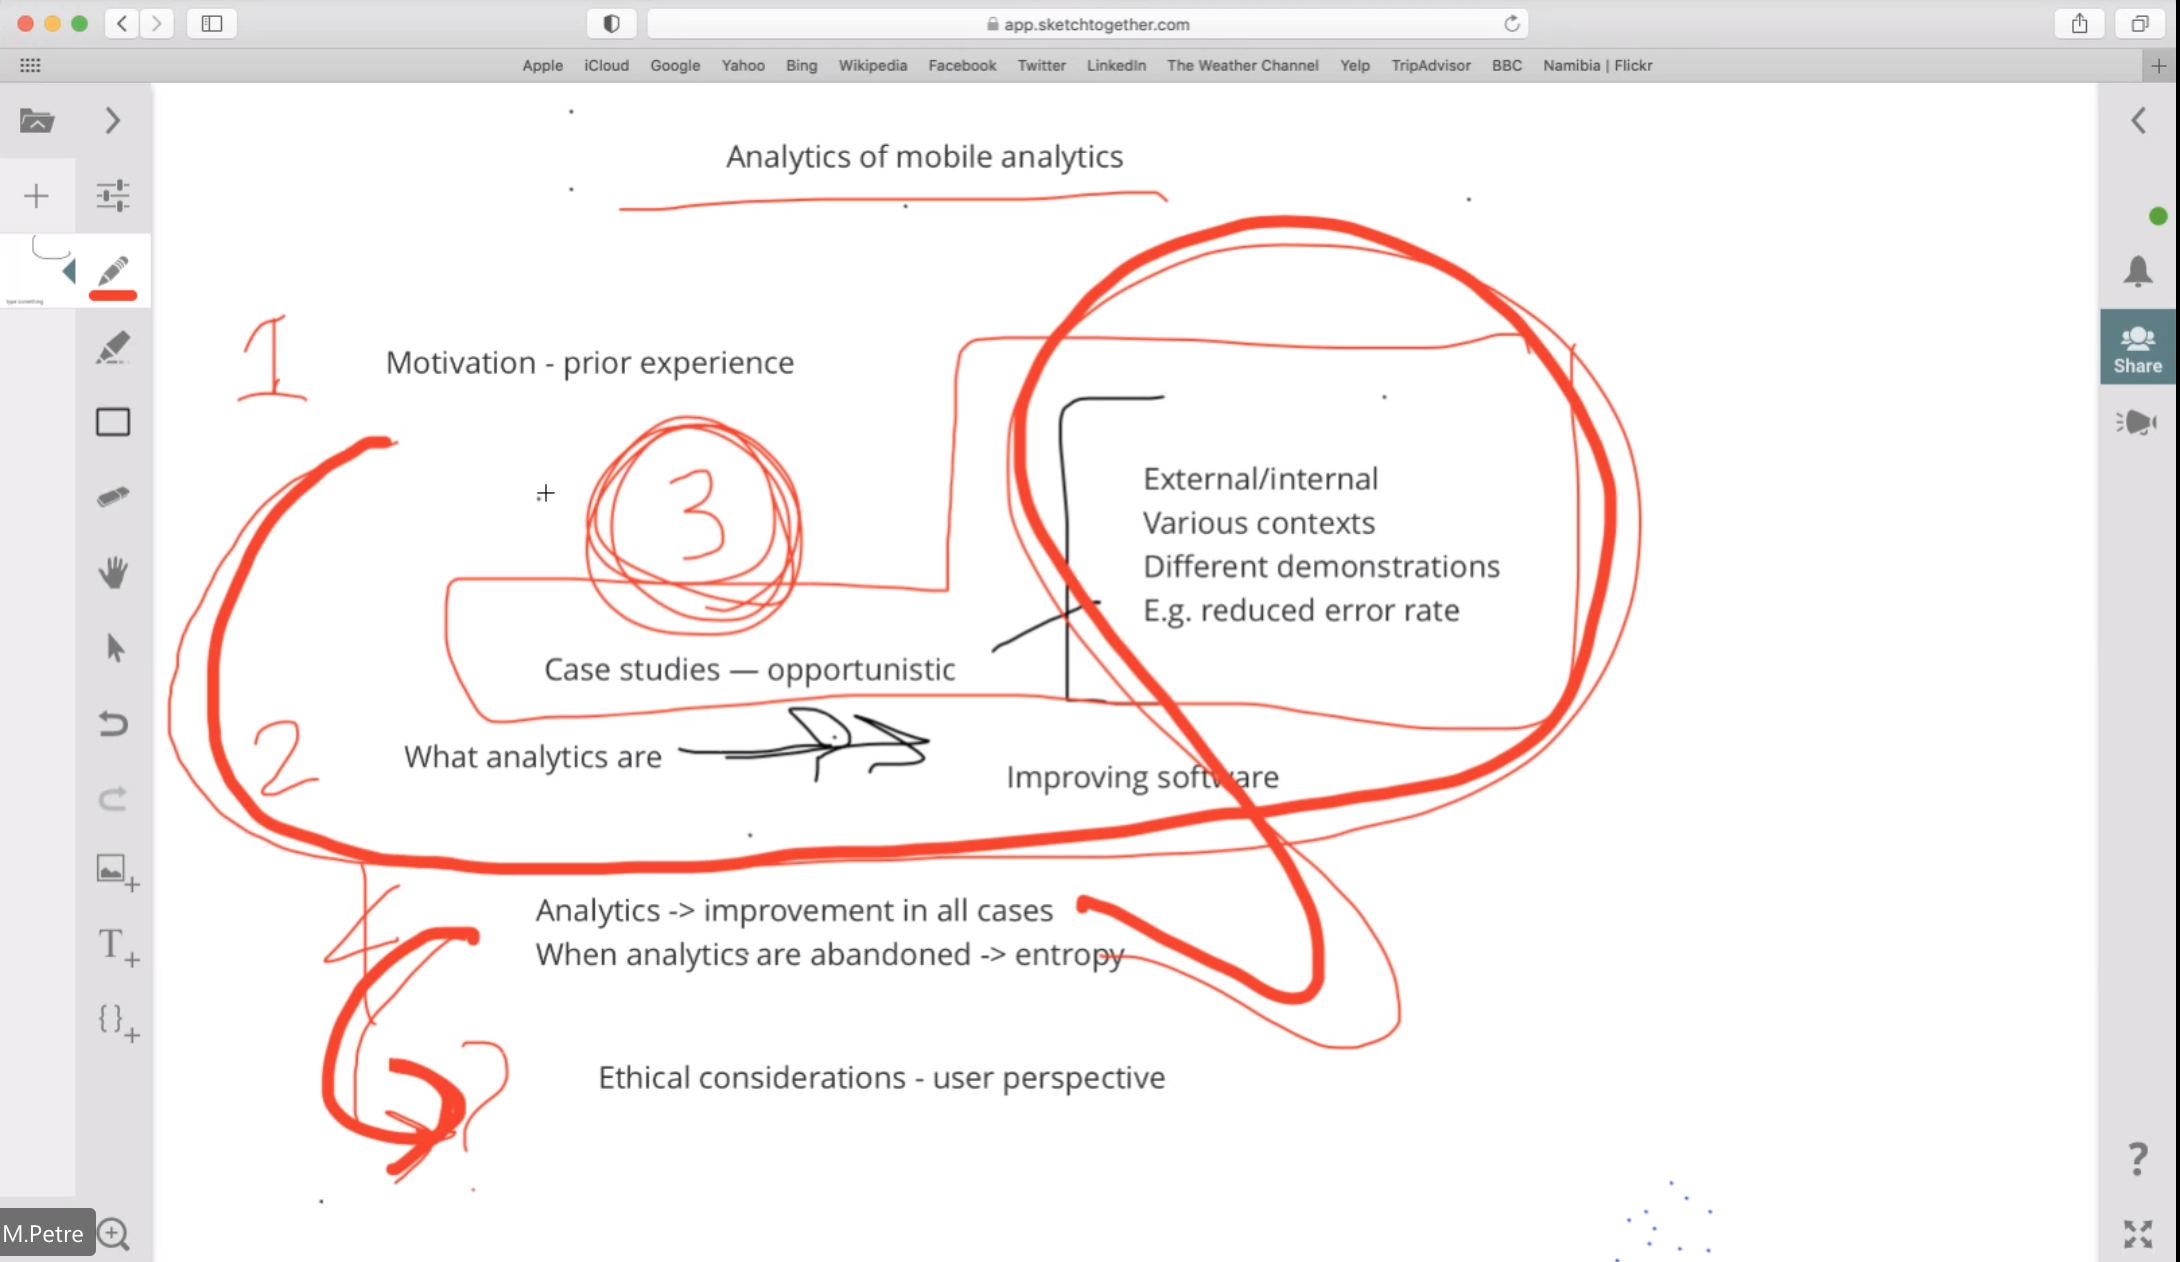
\includegraphics[width=\textwidth]{images/red-thread-pg-forum/marian-red-thread-2021-04-29c.png}
    \caption{Marian's Red Thread sketch~\nth{29} April 2021}
    \label{fig:marians-red-thread-2021-04-21c}
\end{figure}

\begin{mdframed}[style=MyFrame]
[11:26] Ganiat.Kazeem
    
another thing there is to develop understanding of the software engineering practices and approaches
(1 liked)​[11:28] Ganiat.Kazeem
    
highlighting the benefit of understanding analytics,  the potential and varied limitations of analytics depending on source and type, utilising analytics within the software engineering process to understand the problems and institute solutions that prevent entrophy
(1 liked)​[11:29] Ganiat.Kazeem
    
Considering the ethical implications of acquisition of analytical data from external sources and implications for users and software engirneers in the context of ethical ICT
​[11:31] Ganiat.Kazeem
    
Achieved by identifying the impact of analytical data usage through case studies in various settings and exploring and motivating the benefits of and or gains made through active response - i.e improving or tweaking software to unpack and resolve problems such as crashing, issue volume and market positioning

Source <\url{https://teams.microsoft.com/l/message/19:de282fda0ad24a9d9bacd8fd70b7b139@thread.tacv2/1619691994442?tenantId=0e2ed455-96af-4100-bed3-a8e5fd981685&amp;groupId=d428d54e-83c9-442e-a725-663d8c01fcc3&amp;parentMessageId=1602680681312&amp;teamName=PGForum (team)&amp;channelName=General&amp;createdTime=1619691994442}>
\end{mdframed}

For a V2 of the Mobile Analytics Playbook, Antoine proposed an interesting approach A copy of the contents is in the HP AppPulseMobile folder and the email source is in a comment in latex % https://mail.google.com/mail/u/0?ui=2&ik=3d29c9d0f3&view=lg&permmsgid=msg-f%3A1529879579280404426&ser=1

As a follow-up to our discussions, I started to capture a list of all the steps a mobile app (front end) team is going through.

The purpose is to:

-          make sure we are all aware of what a mobile front-end devops framework looks like (self-enablement, tech partnership, etc.)

-          Come up with a solution-driven story that enables HPE reps to identify low-hanging fruit and help customers (buy now) increase their maturity model

 

Here the fundamentals behind it:

-          Build: Everything with a CI, a pipeline and a delivery are the most practical place where devOps starts, and the collaboration starts between the groups.

-          Monitor: Once the app is available on the app stores, all attributes of the user experience are being tracked

-          Optimize: Apply analytics to development and testing, and generate better insight into the business

\subsection{email notes on Google IO talks on Firebase 2016}
% Email source https://mail.google.com/mail/u/0/#search/apppulse+mobile/FMfcgxmQHThNhTMPzbrSXPvcDRktDdnK
\nth{21} May 2016

Yijun,
Thank you very much. I've watched that one \url{https://www.youtube.com/watch?v=tb2GZ3Bh4p8} which provides a good overview, and am now watching one that focuses on testing https://www.youtube.com/watch?v=4fyhgHQYG1U 

Here are some short reminders of topics to consider:
Pre-launch report: crashes, screenshots, and security issues (based on what the app consists of c.f. SafeDK)
Robo Crawler - creates instrumentation tests in Espresso. 
Crash Analytics at 14:00 \url{https://www.youtube.com/watch?v=4fyhgHQYG1U} They discuss clustering (which is interesting and useful)
Firebase Analytics, Audiences, and experiments

Buckets
Breadcrumbs (to traceback from crashes, similar to HP's AppPulse Mobile breadcrumbs).

They're not discussing the use of analytics to help with the testing. 
Speak in a couple of hours, and thanks again for pointing out this key topic.

Julian

PS: I've made some more detailed notes while watching both videos which I've pasted in below:

\textbf{First video (Firebase overview for developers)}
Google Firebase

App quality services

test lab for android

crash analytics

new analytics product

Developer experience matters

Cross Platform

Integrated suite of tools

Firebase console - single home to manage your app

Firebase Analytics

designed for apps

event and user centric

connects across Firebase (features)

Free and unlimited

Main view of all key metrics for your app: activity, revenue from in-app purchases, user engagement, where they’re coming from, distribution of app versions across devices, locations, demographics, user interests, retention. Cohort analytics.

How often a user has made a mistake.

Audiences - groups of users based on behaviours e.g. those who made an in-app purchase. Can take targeted actions.

(Ad) network attribution

Funnels: how many users made it through the tutorial.

Realtime database works when the device is offline, designed to then update from the Google servers.

Hosting your domain on Firebase now f-o-c.

Firebase Storage: handles poor connectivity. Supports Google Edge Caching.

Firebase Remote Config from central to devices - roll out of new features without needing a new app in the app store.

Conditions are used to control how the app behaves for Audience(s) of users (and other options e.g. by device model).

Cloud Test Lab being rebranded - test lab for Android. Tests on most popular devices, run a custom set of instrumentations tests and robotests using a spider of your app. Combine with crash analytics for what you didn’t catch. 

Run a robotest - upload an APK. Demo failed. Pick set of devices and Android versions. Provides screenshots, videos of walking through the app. Exceptions, from running tests shown. 

9.3K of crashes, 119 clusters, then prioritised by number of errors or number of users. Type of iOS version affected, Device affected. 

Integrations with other Google services - Google Play in-app purchases appear directly in the console as do ANR’s flow through to Crash Reporting.

James Tamplin - the techie doing the demo, etc.

Francis Ma 

Growing a business with Firebase.

Acquisition of users, engage users, 

currently high-friction to invite new users. Firebase provides dynamic links custom to the user’s device, checks the app is installed, else downloads the correct app, and then deep links into the relevant section of the app. 

Firebase invites. Drop-in widget for sharing.

AdWords: Universal App Campaigns. 

NPR video: Getting users into the content as quickly as possible.

App behaviour now unpredictable from the user’s perspective as it can be reconfigured remotely. Could be perturbing for some users.

My thought: Can we outsource packages of testing from Firebase? Results should then reintegrate into the product’s dashboard.

\url{isapp.com/io} 

\url{firebase.google.com}

\textbf{Second video (on testing)}

Ahmed Mounir Gad - Product Manager at Firebase Test Lab

Fergus Hurley: on the Google Play Developer Console

Ali Abdelhadi:  Product Manager on Firebase Crash Reporting

Michael Bailey:  Android Engineer at American Express

Iordanis from Shazam

Quality = Success

51\% of 1-star reviews due to stability issues. on Google Play.

Nice bug net image for Monitor. 

Develop->Release->Monitor

Photo of device lab in Google Data Centre. Amazing Infrastructure so you don’t need to buy or maintain devices. Android Studio. CI command line integrations Jenkins, CircleCI and TeamCity.

RoboCrawler. Builds an activity map. Creates a video of the app. Espresso Test Recorder. Launch app on the phone, capture the interactions, builds a fully reusable test script in Espresso. 

@9:40 ish Pre-launch report

crashes, screenshots, and security

screenshots: helps identify usability issues - human detects the layout problems, rather than using automation :(

known vulnerabilities - detected in your codebase. 

60\% of top 1000 apps running alpha & beta channels.

Firebase crash reporting: 13:25  

Build an audience of crashing users

Control it remotely using Remote Config

Monitor errors using Crash Reporting

Send notifications to re-engage: to apologise, and maybe offer a discount to keep the users sweet

Build a test case to retest the fix. Run this before launch of the updated app.

Existing app users:

Shazam

PicCollage

Amex

Foursquare

Skyscanner

KKbox

Lollicam

Busbud

WeMesh

Fabulous

@27 mins Espresso tests with Async behaviour. Not yet supported, considering adding delays even though they know it’s not a good solution. They generate code we have to hack to get working.

@28 mins - discussion on when to run the tests in CI on branches, etc.

Modular SDK to keep size of SDK down.

comparison with old vs new crash reporting. 

Branding Firebase

Can clients enter feedback not just errors using the feedback of Firebase e.g. so a user can report odd behaviour.

Custom identifiers in exceptions: not implemented yet, has some privacy implications, a top request.

Testing an app that uses a camera. Mock the input to the camera in instrumentation tests. But back of camera taped to stop people using the camera to view other apps. The answer wasn’t adequate to solve the testing challenge of video processing of rich videos.

Amex 1000+ instrumentation tests - run in shards. Run tests in parallel with code reviews. 

Any cross-platform examples of success - test lab only for Android. 

cf appium - not supported on the test lab. UI Automator 2.0, Espresso and Robotium are supported.

Login testing supported for Google login flows. They’re adding support for other logins.

Scaling

app popular in Kenya unique devices and OS versions, how do they request these devices in the lab, and how will the test lab scale to Google scale. Google taking care of getting the diversity of devices, and making devices available. 

How do you test remote check deposit e.g. that uses the camera. Amex doesn’t test the app that uses a camera. Split the testing into 2 parts: firing the camera, and then processing the image.

How to get the screenshots - are they automatic? Robo interacts for about 5 mins, takes a screenshot roughly once a second. then optimising looking for screen diffs. Espresso is supported with an API for screenshots. Screenshots only for dummy accounts in pre-launch, no screenshots in live.

What is the role for QA in this environment? no need to spend time on test setup of the environment, etc. Now the QA team can focus on the testing. 

@42 mins Espresso Test Recorder - record your script once and run it in the cloud.


Average crash rate of apps - Google won’t tell which are the crashiest apps. Could investigate how to compare with peers anonymously. 

Quality is more than crashes: NPS. Performance testing they’ll start thinking about. 

Testing the look and feel rather than the functionality - today people can look at the screenshots, Google looking at Accessibility. 

Any Android app can be tested. 


\subsection{New startup launched July 2021}
\url{https://cowboyvc.medium.com/mobile-dev-the-new-standard-for-mobile-development-ff41b8ec3ad6}

\url{https://techcrunch.com/2021/07/14/mobile-dev-launches-with-3m-seed-to-catch-app-issues-pre-production/}
 Gergley knows the CEO.
 
 \subsection{Algorithm Transparency}
 
Algorithmic decision-making systems (ADMs) can affect many people for better or worse~\url{http://algorithmtips.org/2019/01/22/welcome/}. \href{http://www.nickdiakopoulos.com/wp-content/uploads/2011/07/Algorithmic-Accountability-Reporting_final.pdf}{Algorithmic accountability reporting}. See \url{http://algorithmtips.org/resources/} and see the highly related work on \href{glossary-ADMs}{\nameref{glossary-ADMs}} \byshortnameref{glossary-ADMs}. Computer Journalism Lab~\url{https://cj-lab.org/}. See also~\url{https://algorithmwatch.org/en/}


\section{Dan Harmon's story telling circle}
This may be useful to help guide the design of the thesis.

    \begin{itemize}
        \item Get the audience to identify with someone or something, - Give that someone or something some kind of need, - And start changing the circumstances.
        \item Have that someone or something deal with the new circumstances - And find the thing that was needed.
        \item Have that someone or something pay the price of the find - And start heading back toward the original circumstances.
        \item show how those original circumstances have changed as a result.
    \end{itemize}
    \emph{Dan Harmon's story telling circle}



\section{Ontology and Epistemology}~\label{section-ontology-and-episetemology}
This section introduces the theoretical perspective in terms of the ontology and epistemology in terms of using mobile analytics for improving app quality.~\footnote{
\begin{itemize}
    \item Ontology \( \rightarrow \) a theory of `being' (existence).
    \item Epistemology \( \rightarrow \) what we can know about the microcosm/the world and how we can know it (a theory of knowledge).
\end{itemize}

Both these definitions are taken from~\cite{marsh2002skin}. While the article is aimed at social science research, it introduces both topics and their relationships clearly and practically~\footnote{Note: newer versions of the introductory material is published in a book: \href{https://www.macmillanihe.com/page/detail/Theory-and-Methods-in-Political-Science/?K=9781137603517}{\emph{``Theory and Methods in Political Science (\nth{4} Edition)".}}}.
}


\textbf{Note:} This could also be used as a lens for applying analytics.


\section{Testing opensource analytics}
Companies, including PostHog, make much of their analytics software opensource. Establishing independent, testable, and verifiable mechanisms for these tools may help increase their credibility, trustworthiness, and improve the quality of their product offerings. In their early days, according to their strategy, they observed:~\emph{``We’ve grown a lot, but it’s clear that the many of our users use us despite a bad experience - bugs, instability, lots of maintenance or confusing UX."}\url{https://posthog.com/handbook/strategy/strategy}. I love their two word summaries:~\emph{``Nail Funnels"} and \emph{``Nail Diagnosis"}. Their table in the section `What are the needs of our target audience?' might also inspire further research post my PhD.

PostHog state `We will always allow you to benchmark PostHog.'~\url{https://posthog.com/handbook/strategy/business-model} apparently unlike Atlassian (see \url{https://community.developer.atlassian.com/t/about-the-new-software-terms-scent-of-intel-re-performance/24041} and \url{https://news.ycombinator.com/item?id=18103162}.

Their Android code appears to be based on that of Segment \url{https://posthog.com/docs/integrate/client/android} and \url{https://github.com/PostHog/posthog-android/tree/master/posthog-samples/posthog-sample/src/main/java/com/posthog/android/sample}.

\newthought{Would time-machines help?}
If time-machines were available in software development developers might be able to go back in time and repair the current application on the user's mobile device before it was installed on the device. 

Conversely, a time-machine could enable users to return to the time and context when an event such as a failure occurred in order to help the developers understand contributory factors that led up to the failure and the aftermath. 

\newthought{Prior art in time-machines}
\textit{FYI This would be moved to the Related Work chapter}
In 1999, time-machine computing was introduced as a way to help to organise and manage electronic information in computing environments, for instance using a desktop environment - `TimeScape' - that supported time travelling on the computer, and time-casting to restore the context that surrounded the use of a given application~\citep{rekimoto1999_time_machine_computing}. However, that work was limited to a desktop computer environment and has not been maintained. 

\section{Telemetry}
\url{https://mobile.twitter.com/el_bhs/status/1440750741384089608} By Ben Sigelman is well worth reading as are his previous threads. Tradeoffs on verboosity vs cases and queries. Should be part of my work on message/protocol/transmission design.

\section{Persistence vs Ephemera and Ease of Working}
\textbf{Ease of Working} depends in part on the persistence and ease of tracking, sharing and analysing the mobile analytics outputs. Sentry provides the ability to star up to 100 key transactions per team which the team can easily find and access~\footnote{\href{https://docs.sentry.io/product/performance/transaction-summary/\#starring-key-transactions}{Starring Key Transactions}}.

\section{A precursor to the six perspectives}
The following is a precursor to the six perspectives currently being used in the thesis.

\subsection{Four perspectives, in a 2x2 matrix}
A possible way of presenting the perspectives is illustrated in Figure~\ref{fig:four-perspectives} and listed below:
{\footnotesize
\begin{enumerate}
    \itemsep0em
    \item [1] What do app developers say they do? (understand the status quo).
    \item [2] What's possible, how much can we influence?
    \item [3] What does their code tell us? (understand current behaviours in terms of the code that's implemented)~\footnote{NB: it might be useful to reanalyse the projects we studies to identify which ones actively include crash reporting.}.
    \item [4] How can we influence the analytics tool developers?
\end{enumerate}
\begin{figure}
    \centering
    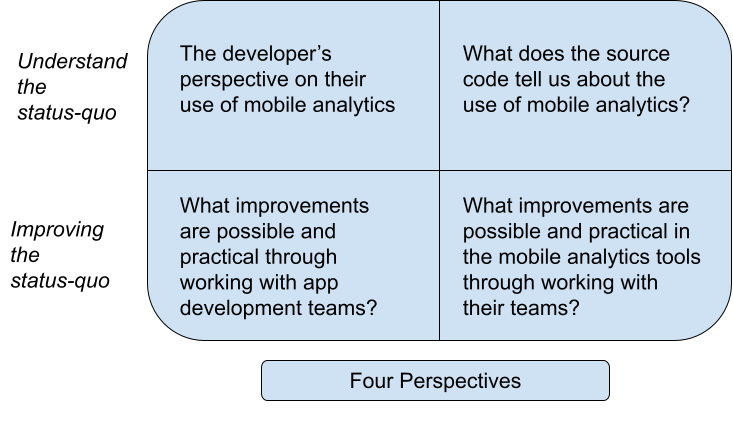
\includegraphics[width=12cm]{images/my/four-perspectives-2x2-matrix.png}
    \caption{Four Perspectives}
    \label{fig:four-perspectives}
\end{figure}
}

These four perspectives distinguish between understanding of the status quo and improving it. However there is a mismatch in the contents of the cells on the right hand side, the upper focuses on the source code of the apps, the lower cell focuses on the mobile analytics tools. This led to the following six perspectives~\footnote{Through discussion with Arosha on \nth{21} Sep 2021.}


\section{Additional considerations}
This section covers several additional topics, including: abandoned apps, additional app stores beyond Google Play and beyond Android, and implications for apps stores for medical devices?

TODO explore the concept that apps `age' and unless they are actively rejuvenated with new releases and the service maintained they risk being abandoned or culled.

\subsection{Abandoned Apps}
Users are not the only people who many abandon apps, developers do so too. By the very nature of abandoning an app a developer is also likely to abandon the reports and data associated with that app, including data from mobile analytics. As many researchers discover there are many abandoned opensource source code repositories, and similarly various organisations, including AppBrain, have identified apps that are effectively abandoned. % MUST-DO add citation for AppBrain report.

\subsection{The Reaper Cometh}
AppBrain is a business that actively monitors and reports on Android Apps in the Google Play Store. The business was founded by two other ex-Google engineers. They state Google is actively culling Android apps from the Google Play store and estimate approximately 16\% of apps are \emph{"low quality apps"} and \emph{"unlikely to be useful"}~\footnote{\url{https://www.appbrain.com/stats/number-of-android-apps}} % Percentage of low quality apps: 16%


\section{Setting the use of mobile analytics in a broader context}

\subsection{Catrobat: Research findings and results from the Case Study}
% Why Catrobat, what did I gain, similarities and contrasts, why include in the PhD.
% Existing best practices, assiduously applied didn't reduce the crash rate, my approach did! :)
% Needs to be applied on a long term basis
